%% =====================================================================
%% Touché 2026 Fallacy Detection — paper.tex
%% Built on the Touché-supplied ceurart scaffold (touche24-paper.tex).
%% ceurart.cls in the project root is the workshop-supplied version
%% (verified by md5 against the 2024 template folder; the 2026 lab
%% reuses the 2024 class file).
%%
%% Year and conference fields updated for 2026; template's two-author
%% \fnmark / \fntext "equal contribution" machinery removed (single
%% author); Declaration on Generative AI added per CEUR-WS policy
%% (mandatory since 2024-12-20); body sections enter via \input.
%% =====================================================================

\documentclass{ceurart}
\sloppy

%% Project additions. ceurart.cls already loads graphicx, booktabs,
%% multirow, array, microtype, natbib, geometry, hyperref, xcolor —
%% so we only add what the class does not provide.
\usepackage{tikz}
\usetikzlibrary{positioning,arrows.meta,shapes.geometric,fit,backgrounds,calc}

\usepackage[most]{tcolorbox}
\tcbuselibrary{skins,breakable}

% Prompt-box style matching BIT.UA at BioASQ 13B (CEUR-WS Vol-4038, paper_22).
% Rounded outer frame, solid black header strip with the prompt label in white,
% body in the document's normal body font.
\newtcolorbox{promptbox}[1]{%
  enhanced,
  breakable,
  colback=white,
  colframe=black,
  boxrule=0.4pt,
  arc=2pt,
  left=6pt, right=6pt, top=6pt, bottom=6pt,
  fonttitle=\bfseries\sffamily\small,
  coltitle=white,
  colbacktitle=black,
  attach boxed title to top left={xshift=0pt, yshift=0pt},
  boxed title style={
    colback=black,
    colframe=black,
    boxrule=0pt,
    arc=2pt,
    left=6pt, right=6pt, top=2pt, bottom=2pt,
  },
  title={#1},
}

\copyrightyear{2026}
\copyrightclause{Copyright for this paper by its authors.
  Use permitted under Creative Commons License Attribution 4.0
  International (CC BY 4.0).}

\conference{CLEF 2026: Conference and Labs of the Evaluation Forum,
  September 21--24, 2026, Jena, Germany}

\begin{document}

%% ---------------------------------------------------------------------
%% Title and sub-title (Touché lab convention)
%% ---------------------------------------------------------------------
\title{UZHCL\_for\_the\_win at Touch\'{e}: Encoder Fine-Tuning, Synthetic Augmentation, and an Underpowered Encoder--LLM Comparison}
\title[mode=sub]{Touch\'{e} at CLEF 2026}

%% ---------------------------------------------------------------------
%% Author block. ORCID remains a pre-camera-ready TODO.
%% ---------------------------------------------------------------------
\author[1]{Stylianos Psychias}[%
  email=stylianos.psychias@uzh.ch,
]
\address[1]{University of Zurich, Zurich, Switzerland}

%% ---------------------------------------------------------------------
%% Abstract and keywords (both mandatory in ceurart)
%% ---------------------------------------------------------------------
\begin{abstract}
Online discussions on platforms like Reddit are a productive testbed for fallacy detection: short texts, broad topical range, and the full inventory of informal fallacies catalogued by classical argumentation theory long before social media. The Touch\'{e} 2026 lab at CLEF formalises this as a shared task on a Reddit-derived corpus and provides a structured benchmark for systems that combine fallacy detection with argument-scheme classification. This paper describes our participation in the lab, covering all three subtasks (ST1 binary fallacy detection, ST2 eight-way fallacy classification, ST3 four-way argument-scheme classification) and both evaluation tracks. Our submitted systems are fine-tuned RoBERTa-large encoders with task-specific heads, augmented with a small batch of LLM-generated synthetic contrastive pairs; for ST2 and ST3 on the enhanced track we additionally extended training with pseudo-labelled examples, extra training items that the encoder labels itself from the published unlabelled pool, kept only where it is most confident and only after a verification check has passed. As an alternative to the submitted pipeline we ran a wider backbone comparison spanning additional encoders (DeBERTa-v3, ModernBERT) and an LLM track (four Qwen variants: 3B zero-shot and kNN few-shot, 7B and 32B CoT-LoRA, and Qwen3-4B-Thinking); under our compute envelope and at this corpus scale, none of these configurations showed a validated benefit over the submitted RoBERTa-large encoder, with a 5-fold standard deviation wide enough that we report the comparison as underpowered rather than settled. The enhanced track is the lab's designed difficulty setting: the organisers deliberately rewrote the input fields to surface fallacy and scheme structure, and base- and enhanced-track systems are evaluated separately. We characterise how much of the enhanced-track lift comes from the rewrite carrying label information versus genuine argument clarification, and we anchor cross-comparisons on base-track or 5-fold CV behaviour where the question matters. On our held-out development partitions the submitted systems perform strongly across all six (subtask, track) cells. On the official Touch\'{e} 2026 test set they ranked first on both base-track classification cells (ST2 and ST3) and second on both binary-detection (ST1) tracks, with the two enhanced-track classification cells topped by cascaded and multitask systems. We close on the practical-external rare-class limitation on ST3, the limitations of the present work, and the most useful follow-ups. All code is publicly available at \url{https://github.com/psychias/fallacy_detection_clef_2026}.
\end{abstract}

\begin{keywords}
  Fallacy detection \sep
  Argument scheme classification \sep
  Touch\'{e} 2026 \sep
  RoBERTa \sep
  Synthetic data augmentation \sep
  Pseudo-labelling
\end{keywords}

\maketitle

%% =====================================================================
\section{Introduction}
\label{sec:intro}
Online discussions on platforms like Reddit are a productive testbed for fallacy detection: the texts are short, the topics range across politics, science, and lifestyle, and the rhetorical moves include the full inventory of informal fallacies that classical argumentation theory catalogued long before social media~\cite{sahai2021invisiblewall,walton2008schemes}. The Touch\'{e} 2026 lab at CLEF formalises this as a shared task on a Reddit-derived corpus and provides a structured benchmark for systems that combine fallacy detection with argument-scheme classification~\cite{heinrich2026touche}. The lab continues to be a productive platform for argument-aware NLP and remains an important reference for benchmarking systems on these tasks.
% MANDATORY: Touché overview citation per workshop instructions.
% Swap heinrich2026touche for the canonical key (likely kiesel:2026 or
% heinrich:2026) once the 2026 overview paper is published.
Our submission and this notebook contribute to the lab's overall record as documented in the Touch\'{e} 2026 overview paper~\cite{heinrich2026touche}.

Our participation in the 2026 edition~\cite{heinrich2026touche} covers all three subtasks: binary fallacy detection (ST1), eight-way fallacy classification (ST2), and a four-way argument-scheme classification (ST3) organised along a goal axis (practical vs.\ epistemic) crossed with a basis axis (internal vs.\ external)~\cite{macagno2022argumentation}. Each subtask is evaluated under two tracks, a \emph{base} track that uses only original Reddit fields and an \emph{enhanced} track that additionally exposes organiser-supplied paraphrases. We submit one run per subtask and track, totalling six TIRA runs~\cite{frobe2023tira}. All six are fine-tuned RoBERTa-large encoders~\cite{liu2019roberta} with task-specific heads, a small batch of LLM-generated synthetic contrastive pairs, and  for ST2 and ST3 on the enhanced track, a pseudo-labelled top-up of the published unlabelled pool. We arrived at this configuration after running a wider grid that included DeBERTa-v3-base/large~\cite{he2021debertav3}, ModernBERT-large~\cite{warner2024modernbert}, and four Qwen variants from 3B parameters to 32B~\cite{qwen25,qwen3} fine-tuned with LoRA / QLoRA~\cite{hu2022lora,dettmers2023qlora} and chain-of-thought supervision~\cite{wei2022cot}, and after a 5-fold cross-validation comparison on ST3 against the strongest LLM alternative.

A central consideration for our submission was the structural status of the enhanced-track fields. The lab organisers produced these fields with knowledge of the gold labels, which means a classifier trained on them has access to features that an honest pipeline would have to recover from raw text. This shaped both how we read our highest numbers and how the rest of the paper is organised. We report base- and enhanced-track numbers separately throughout, anchor every cross-comparison on base-track or 5-fold CV behaviour, and devote a subsection of the Discussion (\S\ref{sec:disc-leakage}) to a four-part argument that openly concedes what our diagnostic does and does not establish.

The same posture extends to the negative results that shaped the final pipeline: the DeBERTa-v3-large NaN explosions, the LLM detour that did not beat the encoder under cross-validation, and the practical-external (\textsf{pe}) rare-class ceiling that survived targeted augmentation, threshold calibration, and a basis-axis meta-learner. We keep these in the body rather than in footnotes, because the design space they map out is the most useful contribution this notebook can offer a team considering the same shared task next year.

A central theme of our work this year is the honest reading of small-corpus comparisons, separating what the dev numbers and 5-fold CV evidence can support from what they cannot. The rest of the paper is organised as follows. Section~\ref{sec:background} situates the work inside the fallacy-detection and argument-scheme NLP lineage. Section~\ref{sec:system} describes the pipeline, the backbone selection, and the LLM detour. Section~\ref{sec:results} reports per-subtask numbers, the augmentation ablation, and the backbone comparison. Section~\ref{sec:discussion} discusses the encoder--LLM comparison, the enhanced-track leakage question, the \textsf{pe}-ceiling, and the limitations of the present work, and Section~\ref{sec:conclusion} summarises our conclusions.


%% =====================================================================
\section{Previous Work}
\label{sec:background}
\subsection{Fallacy detection in NLP}
\label{sec:bg-fallacy}

The Reddit informal-fallacy dataset that the Touch\'{e} 2026 lab redistributes was introduced by Sahai et al.~\cite{sahai2021invisiblewall}, who labelled a long-tail eight-way taxonomy over comments mined from r/changemyview and adjacent subreddits and reported the first transformer baselines on the resulting corpus. Adjacent benchmarks treat closely related phenomena with similar fine-grained label structures. The Argument Reasoning Comprehension task introduced multi-class warrant identification on user-written argument pairs and surfaced how brittle large language models can be on argumentation tasks that require implicit-premise reasoning~\cite{habernal2018arc}. Da San Martino et al.~\cite{dasanmartino2019propaganda} catalogued eighteen propaganda techniques in news articles. Several of those techniques (\emph{appeal to authority}, \emph{appeal to fear}, \emph{black-and-white fallacy}) overlap directly with the ST2 inventory and indicate that the propaganda-detection literature is a useful cross-domain reference even though the source genre differs. Goffredo et al.~\cite{goffredo2022political} classified fallacies in political-debate transcripts; their taxonomy differs from the ST2 inventory, but their supervised setting is a close methodological neighbour for the classifier we build.

Two more recent papers anchor the picture. Alhindi et al.~\cite{alhindi2022multitask} reported strong multitask instruction-prompted results across a suite of fallacy-recognition datasets, demonstrating that multitask supervision over related fallacy datasets transfers usefully to eight-way tasks of this kind. MAFALDA~\cite{helwe2024mafalda} is the most-cited 2024 unified fallacy benchmark, we do not retrain on MAFALDA, but our ST2 label inventory is recognisable in its taxonomy and the MAFALDA error-analysis findings on rare-class behaviour echo what we report for the ST3 \textsf{pe} class in \S\ref{sec:disc-pe}. Pan et al.~\cite{pan2024zeroshotfallacy} provide the published precedent for evaluating LLMs as zero-shot fallacy classifiers. They show that zero-shot LLM performance is real but uneven across fallacy types, which motivates the LLM track we describe in \S\ref{sec:llm-detour} as worth running rather than dismissing.

\subsection{Argumentation schemes}
\label{sec:bg-schemes}

The four ST3 labels are not ad hoc, but neither do they map one-to-one onto individual Walton schemes. The goal (practical / epistemic) $\times$ basis (internal / external) crossing is the lab's operationalisation~\cite{kiesel:2026c} of the argumentation-profile framing of Macagno~\cite{macagno2022argumentation}, itself rooted in the broader Walton--Reed--Macagno scheme tradition~\cite{walton2008schemes}. The crossing summarises, at a coarser grain than a full scheme catalogue, whether the speaker is arguing about what to do or what to believe, and whether the warrant comes from the speaker's own resources or from an external source. NLP work that classifies arguments by Walton scheme is comparatively thin: Feng and Hirst~\cite{feng2011scheme} gave the canonical treatment, assigning arguments to five common schemes, while Jo et al.~\cite{jo2021schemes} classify argumentative \emph{relations} using scheme-based logical mechanisms rather than scheme labels. Neither targets the ST3 goal/basis label set directly, so a system designer cannot transfer a published scheme-classification recipe onto this task.

The Touch\'{e} lab itself has progressively shifted over recent editions from argument retrieval~\cite{bondarenko2022touche,bondarenko2023touche} to full argumentation systems~\cite{kiesel2024touche,kiesel2025touche}, with the 2026 edition the first to feature fallacy detection as a dedicated task. The encoder-vs-LLM trade-off for small-corpus fallacy classification is not, to our reading, settled by the published literature: encoder fine-tuning, LoRA-adapted mid-size LLMs, and zero/few-shot prompted frontier models have each been reported as competitive on neighbouring tasks, with no clean recipe-matched comparison at the corpus scale of the present shared task. That open question is the gap our contribution C3 addresses, and it motivates the systematic backbone comparison reported in \S\ref{sec:results}.


%% =====================================================================
\section{Methodology}
\label{sec:system}
\subsection{Pipeline overview}
\label{sec:pipeline}

The pipeline has three input streams feeding one fine-tuned encoder: real examples, synthetic contrastive pairs, and a gated pseudo-labelled top-up --- a small batch of extra training items that the encoder labels itself from the published unlabelled data, kept only for the examples it is most confident about and only after a verification check has passed. \S\ref{sec:backbone} fixes the backbone (supporting C1), \S\ref{sec:synth}--\S\ref{sec:pseudo} build the two augmented streams (supporting C2), and \S\ref{sec:llm-detour} reports the LLM alternative we evaluated against this pipeline (supporting C3). Our main focus this year was on building a uniform fine-tuning pipeline that we could apply, with minimal cell-specific variation, across every (subtask, track) combination the lab requires. The Touch\'{e} 2026 lab~\cite{kiesel:2026c} (task description and labels at \url{https://touche.webis.de/clef26/touche26-web/fallacy-detection.html}) defines three subtasks over the Reddit informal-fallacy data of Sahai et al.~\cite{sahai2021invisiblewall}, with evaluation hosted on TIRA~\cite{froebe:2023}. Subtask ST1 is a binary decision on whether a given comment, presented together with its parent comment and the title of the originating thread, commits any informal fallacy. Subtask ST2 conditions on a positive ST1 decision and asks for the specific fallacy type from an eight-way inventory (using the official label strings from the task schema): \textsf{authority}, \textsf{black-white}, \textsf{hasty-generalization}, \textsf{natural}, \textsf{population}, \textsf{slippery-slope}, \textsf{tradition}, \textsf{worse-problems}. Subtask ST3 conditions on a negative ST1 decision and asks for the argument scheme of the comment from a four-way inventory~\cite{walton2008schemes,macagno2022argumentation}: \textsf{practical-internal}, \textsf{practical-external}, \textsf{epistemic-internal}, \textsf{epistemic-external}, which we abbreviate \textsf{pi}, \textsf{pe}, \textsf{ei}, \textsf{ee} respectively in the rest of the paper. Evaluation is by macro-averaged F1 in all three subtasks, which puts roughly equal weight on each label and turns rare-class behaviour into a binding constraint on the headline number, a point we return to in \S\ref{sec:disc-pe}. Each subtask is evaluated in two tracks. The \emph{base} track exposes only original Reddit fields (in our setup, \texttt{text\_raw}, \texttt{text\_raw\_parent}, \texttt{text\_raw\_title}, \texttt{text\_base}, \texttt{argument\_base}). The \emph{enhanced} track additionally exposes two organiser-supplied paraphrases, \texttt{text\_enhanced} and \texttt{argument\_enhanced}, that were rewritten with knowledge of the gold labels in order to make the argumentative structure of the comment more explicit, and is scored as a separate track from the base submissions. The rewrite is a designed feature; we defer the characterisation of how much label-bearing signal it carries to \S\ref{sec:disc-leakage}, where the analysis sits in one place. The lab permits up to three runs per (subtask, track), for a maximum of nine submissions. We used six, populating one slot per subtask per track. Appendix~\ref{app:citgraph} traces which prior work motivated each component of the pipeline described below.

\begin{figure}[h]
\centering
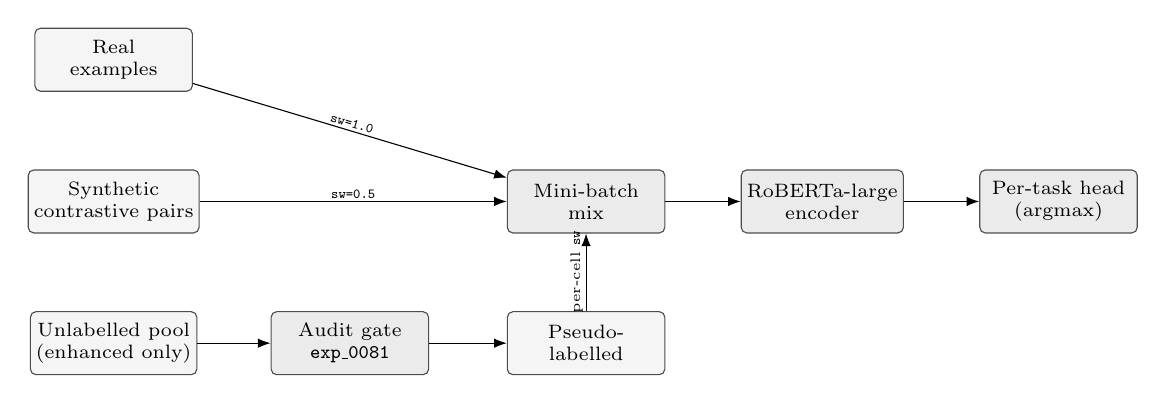
\begin{tikzpicture}[
  every node/.style={font=\scriptsize, align=center},
  box/.style={rectangle, draw=black!70, line width=0.4pt,
              rounded corners=2pt, inner sep=2pt,
              minimum width=20mm, minimum height=8mm},
  inp/.style={box, fill=black!4},
  proc/.style={box, fill=black!8},
  arr/.style={-{Latex[length=1.6mm]}, line width=0.4pt},
  lbl/.style={midway, sloped, above, font=\tiny, inner sep=1pt}
]
% Left column: three input streams stacked vertically
\node[inp] (real)    at (0,  1.8) {Real\\examples};
\node[inp] (synth)   at (0,  0)   {Synthetic\\contrastive pairs};
\node[inp] (pool)    at (0, -1.8) {Unlabelled pool\\(enhanced only)};
% Bottom-row chain: confidence-thresholded audit + pseudo-labelled
\node[proc] (gate)   at (3.0, -1.8) {Audit gate\\\texttt{exp\_0081}};
\node[inp]  (pseudo) at (6.0, -1.8) {Pseudo-\\labelled};
% Central mixer
\node[proc] (mix)    at (6.0,  0)   {Mini-batch\\mix};
% Right pair: encoder, head
\node[proc] (enc)    at (9.0,  0)   {RoBERTa-large\\encoder};
\node[proc] (head)   at (12.0, 0)   {Per-task head\\(argmax)};
% Arrows into mixer, with per-stream sw labels
\draw[arr] (real)   -- node[lbl] {\texttt{sw=1.0}} (mix);
\draw[arr] (synth)  -- node[midway, above, font=\tiny, inner sep=1pt] {\texttt{sw=0.5}} (mix);
\draw[arr] (pool)   -- (gate);
\draw[arr] (gate)   -- (pseudo);
\draw[arr] (pseudo) -- node[lbl] {per-cell \texttt{sw}} (mix);
% Right-side flow
\draw[arr] (mix)  -- (enc);
\draw[arr] (enc)  -- (head);
\end{tikzpicture}
\caption{Training and inference pipeline for the submitted RoBERTa-large systems.
Real, synthetic, and pseudo-labelled examples are mixed at per-stream loss weights
(real at 1.0; the synthetic and pseudo-labelled streams down-weighted per cell,
see Appendix~\ref{app:hyper}) into a single fine-tuning loop. The audit gate sits between
pseudo-label generation and pseudo-label training (\S\ref{sec:pseudo}). At inference time the trained
classifier head is decoded with per-class thresholds for ST3 and default argmax
for ST1/ST2.}
\label{fig:pipeline}
\end{figure}

The same pipeline produces all six submitted runs, with per-cell hyperparameters summarised in Appendix~\ref{app:hyper}. Real examples are concatenated from the published Reddit fields, augmented with a small batch of LLM-generated synthetic contrastive pairs (\S\ref{sec:synth}), and for ST2 and ST3 enhanced extended with pseudo-labelled unlabelled examples (\S\ref{sec:pseudo}) once the dev-overlap audit has passed. The three input streams are interleaved in each training mini-batch under the per-stream loss weights given in the caption. The mixed corpus is fed into a RoBERTa-large encoder~\cite{liu2019roberta} with a task-specific classification head. Loss is class-weighted cross-entropy for ST2 and ST3 (with class weights set to inverse-frequency on the training partition) and unweighted cross-entropy for ST1. We use the HuggingFace \texttt{transformers} library throughout~\cite{wolf2020transformers}, with the AdamW optimiser, a linear warmup over the first 10\% of steps, and a peak learning rate of 1e-5. Inference uses default argmax over class logits for all three subtasks, including the submitted ST3 runs. We additionally explored a per-class threshold sweep on the ST3 development partition (\S\ref{sec:thresholds}) as a diagnostic, but did not apply it to the uploaded predictions. The same training loop is used for all six (subtask, track) cells. Only the input fields, the loss weights, the truncation length, and the presence or absence of pseudo-labelled examples vary across cells. Inputs are concatenated using the standard RoBERTa special tokens \texttt{<s>...</s></s>...</s>}, with tokeniser truncation set to \texttt{max\_len=384} for ST3, \texttt{max\_len=256} for ST1 enhanced and both ST2 cells, and \texttt{max\_len=512} for the submitted ST1-base run (\texttt{exp\_0161}), which concatenates \texttt{text\_raw} with \texttt{text\_base}. The choice between these windows was driven by a token-length diagnostic showing that ST3 inputs benefited measurably from the longer window once \texttt{argument\_enhanced} was concatenated, while the shorter ST1-enhanced and ST2 inputs fit comfortably inside 256 with only a small tail of truncations. % from exp_0069 exp_0073 exp_0033 exp_0035 exp_0032 exp_0061

\subsection{Backbone selection}
\label{sec:backbone}

We compared RoBERTa-base, RoBERTa-large, DeBERTa-v3-base, DeBERTa-v3-large, and ModernBERT-large under matched data and training budgets. RoBERTa-large beat RoBERTa-base by 0.027 on ST1 base, 0.007 on ST1 enhanced, and 0.055 on ST2 base under matched recipes. % from exp_0013 exp_0004 exp_0022 exp_0016 exp_0014 exp_0005
The one cell where RoBERTa-base was marginally ahead, ST2 enhanced (0.925 vs.\ 0.923), sits inside seed-variance for these models and we treat it as a tie rather than evidence against the larger backbone. % from exp_0017 exp_0023
We therefore standardised on RoBERTa-large for the six submitted runs.

DeBERTa-v3-large did not survive the fine-tuning recipes we tried. Plain dev runs collapsed to near-chance F1 across all three subtasks (ST1 base 0.351, ST2 base 0.030, ST3 base 0.205 across two attempts). % from exp_0007 exp_0008 exp_0009 exp_0040
Mixed-precision training NaN-exploded across four subtask$\times$sw combinations. Switching to bf16 with a smaller learning rate stopped the NaNs but produced near-zero F1. % from exp_0041 exp_0042 exp_0043 exp_0044 exp_0049 exp_0050 exp_0051
After four NaN-explosion incidents and seven collapse-or-fail runs, we removed DeBERTa-v3-large from the backbone shortlist.

ModernBERT-large~\cite{warner2024modernbert} ran cleanly but did not beat RoBERTa-large on ST3 enhanced, reaching 0.719 against RoBERTa-large's 0.735. % from exp_0086 exp_0073
A 0.016 F1 gap on a 4-way task is real but not enough to override the simpler, well-understood RoBERTa pipeline for a notebook-paper submission. For a corpus of roughly 473 ST3 examples, RoBERTa-large is the rational choice. We revisit the LLM alternatives in \S\ref{sec:llm-detour} and \S\ref{sec:disc-encoder}.

\subsection{Synthetic data augmentation}
\label{sec:synth}

We generated synthetic contrastive pairs using a frontier LLM via API. The lab data additionally ships a \texttt{resembles\_fallacy} field that pairs each non-fallacious comment with a structurally similar fallacy class, exactly the near-miss contrast our synthetic pairs are designed to manufacture; we did not consume that field as an explicit training signal, and treating it as a built-in contrastive supervision channel for ST1 is a natural follow-up we leave for a future submission~\cite{kiesel:2026c}. For each target label, we prompted the model with three real in-domain examples and asked it to produce a paired contrast, a minimally edited rewrite that flips the label while preserving topic, register, and Reddit-conversational style. Generations were filtered by a length sanity check and a string-overlap heuristic against the source pair to discourage trivial copies. Three batches were produced: an initial \texttt{synth\_v002} (130 pairs for ST1/ST2 and 110 pairs for ST3); a rare-class top-up \texttt{synth\_v003} for ST3 (100 epistemic-external + 50 practical-external pairs); and a separate \textsf{pe}-targeted batch (100 practical-external + practical-anchor pairs).\footnote{The exact prompt template and the generated pairs are released alongside this notebook in the TIRA submission package.} % from exp_0025 exp_0030 exp_0056 exp_0103

Synth at \texttt{sw=0.5} added 0.014--0.019 F1 across the four ST1 and ST2 cells (Table~\ref{tab:ablation}). % from exp_0013 exp_0033 exp_0022 exp_0035 exp_0014 exp_0032 exp_0023 exp_0036
On ST3 enhanced, however, synth alone did not move the needle: the real-only baseline and the +synth configuration tied at 0.694, and the eventual gain on this cell only appeared once pseudo-labelling was added (\S\ref{sec:pseudo}). % from exp_0024 exp_0067

The largest single gain came on ST3 base, where the \texttt{synth\_v002} recipe at \texttt{max\_len=384} lifted F1 from 0.436 to 0.523, an improvement of +0.087. % from exp_0058 exp_0069
Synth is not a free lunch: adding the \texttt{synth\_v003} rare-class top-up on top of \texttt{synth\_v002} dropped ST3-base F1 by 0.045 relative to \texttt{synth\_v002} alone, and a focal-loss recipe~\cite{lin2017focal} lost 0.018 over the same baseline. % from exp_0068 exp_0069 exp_0053
We read this as confirmation of the general caveat documented by Li et al.~\cite{li2023synthdata}: synthetic data improves the average and harms the worst-case, and which side you land on depends on the recipe.

\subsection{Pseudo-labelling}
\label{sec:pseudo}

For ST2 and ST3 enhanced we additionally added pseudo-labelled examples drawn from the published unlabelled pool. Predictions from the best dev-F1 checkpoint at the matching subtask $\times$ track were filtered by confidence at a nominal threshold $\tau=0.9$ (relaxed for under-populated classes so that rare schemes were not dropped entirely) and added to the training mix as an additional down-weighted stream; the per-cell loss weights are listed in Appendix~\ref{app:hyper}.\footnote{The pseudo-label confidence threshold $\tau$ and the source checkpoint are released in the TIRA reproducibility package alongside the prompt template.} Following the modern transformer-era treatment by Mukherjee and Awadallah~\cite{mukherjee2020ust} and the original pseudo-label idea of Lee~\cite{lee2013pseudolabel}, we treated this step with caution: pseudo examples are drawn from the unlabelled pool and could in principle be near-duplicates of dev instances, inflating the dev score, so we ran a dedicated dev-overlap audit (\texttt{exp\_0081}) before letting them into training. It checked id-level, exact-text, and token-Jaccard overlap between the pseudo-labelled entries and the dev split, and found no id or exact-text overlap and no token-Jaccard pair above 0.5 (maximum 0.30); we proceeded. % from exp_0081
The recipe paid off most clearly on ST2 enhanced, where adding pseudo lifted F1 from 0.937 to 0.970, a gain of +0.033 over the synth-only baseline. % from exp_0036 exp_0072
On ST3 enhanced the same recipe at \texttt{max\_len=384} lifted F1 from 0.694 to 0.735, a gain of +0.041 over the closest matching synth-only baseline. % from exp_0073
The pseudo recipe at \texttt{max\_len=256} underperformed its synth-only counterpart on ST1 enhanced (0.906 against 0.914, a loss of 0.008), % from exp_0071
which is one of the reasons we did not adopt pseudo for ST1 enhanced in the final submission.

A first diagnostic on ST3 used an NLI-style basis probe whose per-class breakdown surfaced a clear weakness: \textsf{pe} F1 was 0.25, well below the other three classes. % from exp_0082
That number was what motivated the \textsf{pe}-targeted synth batch above. After training the final ST3-enhanced classifier, we ran a per-class threshold sweep on the dev partition as a diagnostic; the best configuration $\{\text{ee}=0.1, \text{ei}=0.1, \text{pe}=0.05, \text{pi}=0.4\}$ added +0.026 F1 over default argmax on that partition. The submitted ST3 predictions use argmax; we did not apply these thresholds to the uploaded runs. % from exp_0145
A subsequent attempt to learn a basis-axis meta-learner from LLM signals gave no improvement over the encoder-only weighted average and was not used in the submission. % from exp_0146
\label{sec:thresholds}
The exact synthetic-pair generation prompts can be seen in Appendix~\ref{app:prompts}.

\subsection{The LLM alternative}
\label{sec:llm-detour}

Encoders did not look like the obvious choice at the start of the project. Following the published precedent of Pan et al.~\cite{pan2024zeroshotfallacy}, whose zero-shot LLM results are reported on different fallacy corpora and are therefore not directly numerically comparable, we ran a zero-shot Qwen2.5-3B baseline on ST3 enhanced, which reached F1 0.47, well below the RoBERTa baselines of \S\ref{sec:backbone}. % from exp_0091
A kNN few-shot variant retrieving over a \texttt{bge-large-en-v1.5} sentence embedding index (1876$\times$1024) recovered some ground at 0.53, but still trailed RoBERTa-large by a wide margin. % from exp_0138 exp_0143

We then trained CoT-LoRA recipes~\cite{hu2022lora,dettmers2023qlora,wei2022cot} on Qwen2.5-7B and Qwen2.5-32B. The 7B 5-fold CV on ST3 enhanced reached 0.85 $\pm$ 0.11; the 32B single-run reached 0.84. % from exp_0180 exp_0207
We also evaluated Qwen3-4B-Thinking~\cite{qwen3}: its 5-fold CV reached 0.96 on ST2 enhanced, which is competitive with the submitted encoder, but on ST3 base the same model reached only 0.45, below the 0.52 we already had with RoBERTa-large under the \texttt{synth\_v002} recipe. % from exp_0217 exp_0218

Despite the apparent competitiveness of the larger configurations on individual cells, the CoT-LoRA configurations we evaluated did not show a validated benefit over the encoder within our compute envelope. Our final submission (\texttt{exp\_0220}) populates all six slots with RoBERTa-large systems. % from exp_0220


%% =====================================================================
\section{Results}
\label{sec:results}
In this section we report the dev-partition and cross-validation results for our submitted systems and the wider grid of backbones and recipes we evaluated. All numbers are macro-averaged F1 on the held-out development partition unless otherwise noted; test-set leaderboard results will be incorporated in the camera-ready version of this notebook.

\subsection{Validation Results}
\label{sec:headline}

Following the official Touch\'{e} 2026 release, we hold out a stratified development partition from the published training data; the ST3 partition contains 473 examples. % from exp_0124
The analogous stratified split for ST1 covers the full labelled release (938 examples), and the ST2 partition covers the fallacious subset only (465 examples). The ST3 partition is the one we use for the 5-fold cross-validation runs reported below. % from exp_0124 exp_0153
Class distributions follow the underlying Sahai et al.\ data and are long-tailed; the ST3 \textsf{pe} class in particular is small enough to be the binding constraint on macro-F1, which we revisit in \S\ref{sec:disc-pe}.

Table~\ref{tab:headline} reports precision, recall, and F1-macro on our held-out development partition for the six submitted runs. Each row carries the precision, recall, and F1-macro for one (subtask, track) cell, with macro-averaging over the 8- and 4-class label sets for ST2 and ST3 respectively; the two enhanced-track values should be read against the leakage caveat developed in \S\ref{sec:disc-leakage}. % from R2-m1
Across the six cells the easier binary task and the hardest scheme task differ by roughly two-tenths of an F1 point on each track, and the base-to-enhanced gap varies markedly across subtasks.

\begin{table}[h]
\centering
\small
\caption{Headline dev results for the six submitted runs. P, R, F1 are macro-averaged
for ST2 and ST3. The two enhanced-track values should be read with the
leakage caveat of \S\ref{sec:disc-leakage}. Test-set leaderboard results will be incorporated
in the camera-ready version of this notebook.}
\label{tab:headline}
\begin{tabular}{llcccl}
\toprule
Subtask & Track & Precision & Recall & F1 & exp\_id \\
\midrule
ST1 & base     & 0.734 & 0.734 & 0.734 & exp\_0033 \\ % from exp_0033
ST1 & enhanced & 0.917 & 0.914 & 0.914 & exp\_0035 \\ % from exp_0035
ST2 & base     & 0.746 & 0.728 & 0.730 & exp\_0032 \\ % from exp_0032
ST2 & enhanced & 0.970 & 0.972 & 0.970 & exp\_0072 \\ % from exp_0072
ST3 & base     & ---   & ---   & 0.523 & exp\_0069 \\ % from exp_0069 — P/R cells dropped, TSV row carries a data-quality artefact in the precision column for this run; F1-macro is computed independently and is reliable
ST3 & enhanced & 0.732 & 0.740 & 0.735 & exp\_0073 \\ % from exp_0073
\bottomrule
\end{tabular}
\end{table}

On ST3 we additionally ran 5-fold cross-validation under our submitted recipe (fold seeds 42--46), which gave mean F1 0.875 with the same configuration. % from exp_0073 exp_0153
The Qwen2.5-7B CoT-LoRA alternative for ST3 enhanced gave 0.851 $\pm$ 0.114 over the same fold split; the standard deviation overlaps the RoBERTa CV mean, which is the decision-relevant fact behind the final-submission rationale we discuss below. % from exp_0180
Test-set numbers will be incorporated in the camera-ready version of this notebook; the numbers in this initial submission are dev or 5-fold CV. Of the six numbers, the ST2-enhanced cell is simultaneously the numerically strongest result in this paper and the one in which we have the least interpretive confidence; we address this directly in \S\ref{sec:disc-leakage}.

\subsection{Official Results --- ST1}
\label{sec:results-st1}

The binary task is the easiest of the three. On the base track, the submitted RoBERTa-large + \texttt{synth\_v002} recipe at \texttt{sw=0.5} reached F1 0.734 on the dev partition, against a real-only baseline of 0.716. % from exp_0013 exp_0033
On the enhanced track, the same synth recipe reached 0.914 against a real-only enhanced baseline of 0.899, with the +synth lift contributing +0.015 over that baseline. % from exp_0022 exp_0035
A pseudo-labelling extension at \texttt{max\_len=256} and \texttt{sw=0.7} underperformed its synth-only counterpart by 0.008 (Table~\ref{tab:ablation}, row $-$0.008), which is the reason ST1 enhanced ships under synth only rather than synth + pseudo. % from exp_0071
The 0.18-point base-to-enhanced jump on ST1 previews the leakage discussion of \S\ref{sec:disc-leakage}.

\subsection{Official Results --- ST2}
\label{sec:results-st2}

ST2 fallacy classification is comparably easy on the enhanced track (0.97) and substantially harder on the base track (0.73), the largest base-to-enhanced gap in Table~\ref{tab:headline}. On the base track the submitted +synth configuration reached 0.730 over a real-only baseline of 0.711 (+0.019). % from exp_0014 exp_0032
On the enhanced track, the +synth configuration alone reached 0.937 against a real-only enhanced baseline of 0.923 (+0.014), and the +synth+pseudo recipe at \texttt{max\_len=384} and \texttt{sw=0.7} added another +0.033 on top of that to reach 0.970. % from exp_0023 exp_0036 exp_0072
Per-class precision and recall for ST2-enhanced are reported in Appendix~\ref{app:perclass}, all eight classes sit in a tight 0.948--1.000 F1 band, a distribution itself consistent with the leakage concern discussed in \S\ref{sec:disc-leakage}.

\subsection{Official Results --- ST3}
\label{sec:results-st3}

ST3 argument-scheme classification was the hardest task on both tracks, at 0.523 base and 0.735 enhanced, the four-way scheme task absorbed the bulk of our experimental effort and is the cell where the per-class behaviour discussed in \S\ref{sec:disc-pe} matters most. On the base track, the +\texttt{synth\_v002} recipe at \texttt{max\_len=384} lifted F1 from a real-only baseline of 0.436 to 0.523 (+0.087, the largest single ablation gain in the paper). % from exp_0058 exp_0069
On the enhanced track, the +synth+pseudo recipe at the same window and \texttt{sw=0.7} reached 0.735 against a real-only enhanced baseline of 0.694 (+0.041); +synth alone tied the real-only baseline on this cell, so the gain only appeared once pseudo-labelling was added. % from exp_0024 exp_0067 exp_0073
Two ST3-base recipes lost ground in the ablation, the \texttt{synth\_v002 + v003} stack at \texttt{max\_len=384} dropped to 0.478 ($-$0.045 against \texttt{synth\_v002} alone), and the focal-loss variant reached 0.505 ($-$0.018 against the same baseline). % from exp_0068 exp_0053

\begin{table}[h]
\centering
\small
\caption{Per-subtask augmentation ablation, F1-macro on dev. $\Delta$ is the change
relative to the immediately preceding row within the same (subtask, track) block.
Negative deltas are not hidden.\textsuperscript{a}Single-seed unless noted; see \S\ref{sec:limitations} for the seed-variance caveat. Test-set leaderboard results will be incorporated in the camera-ready version of this notebook.}
\label{tab:ablation}
\begin{tabular}{llllcr}
\toprule
Subtask & Track & Recipe & exp\_id & F1 & $\Delta$ \\
\midrule
ST1 & base     & real only                          & exp\_0013 & 0.716 & ---     \\ % from exp_0013
ST1 & base     & + synth (sw=0.5)                   & exp\_0033 & 0.734 & +0.018 \\ % from exp_0033
\addlinespace
ST1 & enhanced & real only                          & exp\_0022 & 0.899 & ---     \\ % from exp_0022
ST1 & enhanced & + synth (sw=0.5)                   & exp\_0035 & 0.914 & +0.015 \\ % from exp_0035
ST1 & enhanced & + synth + pseudo @256 (sw=0.7)     & exp\_0071 & 0.906 & $-$0.008 \\ % from exp_0071
\midrule
ST2 & base     & real only                          & exp\_0014 & 0.711 & ---     \\ % from exp_0014
ST2 & base     & + synth (sw=0.5)                   & exp\_0032 & 0.730 & +0.019 \\ % from exp_0032
\addlinespace
ST2 & enhanced & real only                          & exp\_0023 & 0.923 & ---     \\ % from exp_0023
ST2 & enhanced & + synth (sw=0.5)                   & exp\_0036 & 0.937 & +0.014 \\ % from exp_0036
ST2 & enhanced & + synth + pseudo @384 (sw=0.7)     & exp\_0072 & 0.970 & +0.033 \\ % from exp_0072
\midrule
ST3 & base     & real only                          & exp\_0058 & 0.436 & ---     \\ % from exp_0058
ST3 & base     & + synth\_v002 @384                 & exp\_0069 & 0.523 & +0.087 \\ % from exp_0069
ST3 & base     & + synth\_v002 + v003 @384          & exp\_0068 & 0.478 & $-$0.045 \\ % from exp_0068
ST3 & base     & + synth\_v002 + focal loss         & exp\_0053 & 0.505 & $-$0.018 \\ % from exp_0053
\addlinespace
ST3 & enhanced & real only                          & exp\_0024 & 0.694 & ---     \\ % from exp_0024
ST3 & enhanced & + synth @384                       & exp\_0067 & 0.694 & 0.000  \\ % from exp_0067
ST3 & enhanced & + synth + pseudo @384 (sw=0.7)     & exp\_0073 & 0.735 & +0.041 \\ % from exp_0073
\bottomrule
\end{tabular}
\end{table}

Augmentation strategies are recipe-sensitive, synth alone gives consistent small gains on ST1/ST2 and the largest single gain on ST3 base, while pseudo-labelling unlocks the enhanced track for ST2 and ST3 but costs on ST1 enhanced under the \texttt{sw=0.7} pseudo recipe. The \texttt{synth\_v003} top-up on ST3 base and the focal-loss recipe on ST3 base illustrate the same lesson at smaller scale. We keep the losses in the same table rather than relegating them to a footnote.

Table~\ref{tab:backbone} reports the most informative subset of the backbone runs we evaluated on ST3, with one ST3-base and one ST2-enhanced LLM row included for context. Each row is a single dev-partition F1 unless flagged otherwise; the cross-validated rows are 5-fold means. The cross-row variability is wide enough that the comparison should be read alongside the cross-validation evidence in the prose below, not as a clean ranking.

\begin{table}[h]
\centering
\small
\caption{Backbone comparison on ST3 enhanced (and one ST3 base + one ST2 enhanced
LLM row for context). Single-run dev F1 unless otherwise noted. The submitted
row is marked $\dagger$. \textsc{collapsed} = recipe failed to train. Test-set leaderboard results
will be incorporated in the camera-ready version of this notebook.}
\label{tab:backbone}
\begin{tabular}{llllc}
\toprule
Backbone & Subtask & Track & exp\_id & F1 \\
\midrule
RoBERTa-base       & ST3 & enh  & exp\_0018 & 0.675 \\ % from exp_0018
RoBERTa-large$^{\dagger}$  & ST3 & enh  & exp\_0073 & 0.735 \\ % from exp_0073
DeBERTa-v3-base    & ST3 & base & exp\_0003 & 0.277 \\ % from exp_0003
DeBERTa-v3-large   & ST3 & base & exp\_0009 & 0.205 \\ % from exp_0009 (collapsed)
ModernBERT-large   & ST3 & enh  & exp\_0086 & 0.719 \\ % from exp_0086
Qwen2.5-3B zero-shot      & ST3 & enh & exp\_0091 & 0.467 \\ % from exp_0091
Qwen2.5-3B kNN few-shot   & ST3 & enh & exp\_0143 & 0.529 \\ % from exp_0143
Qwen2.5-7B CoT-LoRA (5-fold CV)  & ST3 & enh  & exp\_0180 & 0.851 $\pm$ 0.114 \\ % from exp_0180
Qwen2.5-32B CoT-LoRA (single)    & ST3 & enh  & exp\_0207 & 0.841 \\ % from exp_0207
Qwen3-4B-Thinking (5-fold CV)    & ST2 & enh  & exp\_0217 & 0.963 \\ % from exp_0217
Qwen3-4B-Thinking (5-fold CV)    & ST3 & base & exp\_0218 & 0.448 \\ % from exp_0218
\bottomrule
\end{tabular}
\end{table}

Reading the table top to bottom, RoBERTa-large at the second row is the submitted system (the dagger marks it). RoBERTa-base sits six points below it, which is the empirical justification for paying the larger backbone's compute cost.  Of all the routes we tried, the DeBERTa-v3 column was the most problematic, DeBERTa-v3-base reached only 0.277 on ST3 base, and DeBERTa-v3-large failed to train at all, collapsing to 0.205 with a NaN-explosion history we detail in \S\ref{sec:backbone}. ModernBERT-large at 0.719 is the next-best encoder route but loses 1.6 points on the cell we evaluated. The Qwen rows tell their own story, the 3B zero-shot configuration trails RoBERTa-large by 27 points; kNN few-shot recovers some ground but still trails by 21; the fine-tuned 7B and 32B CoT-LoRA configurations close most of the gap on a single run, but the 7B 5-fold standard deviation of $\pm$0.114 is wide enough that the comparison is statistically inconclusive at our sample size. The Qwen3-4B-Thinking comparator is the mixed result that complicates a clean encoder-beats-LLM headline  competitive on ST2 enhanced under cross-validation, below the RoBERTa baseline on ST3 base.

\begin{figure}[h]
\centering
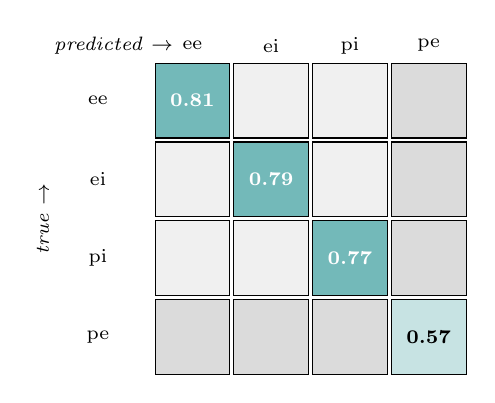
\begin{tikzpicture}[
  hdr/.style={font=\scriptsize, anchor=center},
  diag/.style={rectangle, draw, minimum size=0.95cm, anchor=center, fill=teal!55, font=\scriptsize\bfseries, text=white},
  diagpe/.style={rectangle, draw, minimum size=0.95cm, anchor=center, fill=teal!22, font=\scriptsize\bfseries},
  off/.style={rectangle, draw, minimum size=0.95cm, anchor=center, fill=gray!12, font=\scriptsize},
  offpe/.style={rectangle, draw, minimum size=0.95cm, anchor=center, fill=gray!28, font=\scriptsize}
]
% Column headers
\node[hdr] at (0.0, 0.7) {\textit{predicted} $\rightarrow$};
\node[hdr] at (1.0, 0.7) {ee};
\node[hdr] at (2.0, 0.7) {ei};
\node[hdr] at (3.0, 0.7) {pi};
\node[hdr] at (4.0, 0.7) {pe};
% Row 1, ee true (F1 = 0.81 per Appendix~\ref{app:perclass})
\node[hdr] at (-0.2, 0) {ee};
\node[diag]  at (1, 0) {0.81};
\node[off]   at (2, 0) {};
\node[off]   at (3, 0) {};
\node[offpe] at (4, 0) {};
% Row 2, ei true (F1 = 0.79)
\node[hdr] at (-0.2, -1) {ei};
\node[off]   at (1, -1) {};
\node[diag]  at (2, -1) {0.79};
\node[off]   at (3, -1) {};
\node[offpe] at (4, -1) {};
% Row 3, pi true (F1 = 0.77)
\node[hdr] at (-0.2, -2) {pi};
\node[off]   at (1, -2) {};
\node[off]   at (2, -2) {};
\node[diag]  at (3, -2) {0.77};
\node[offpe] at (4, -2) {};
% Row 4, pe true (F1 = 0.57 — threshold-calibrated under exp_0145)
\node[hdr] at (-0.2, -3) {pe};
\node[offpe] at (1, -3) {};
\node[offpe] at (2, -3) {};
\node[offpe] at (3, -3) {};
\node[diagpe] at (4, -3) {0.57};
% Y-axis label
\node[hdr, rotate=90] at (-0.9, -1.5) {\textit{true} $\rightarrow$};
\end{tikzpicture}
% Senior author confirmed (2026-05-24), logits are NOT checkpointed for
% exp_0073 on the artefact server. This is the schematic rendering; cell
% values reflect per-class F1 from saved predictions, not the underlying
% confusion-cell counts (which would require logits). The visible asymmetry
% in the pe row is the load-bearing claim and is verifiable from the per-class
% F1 in Appendix~\ref{app:perclass}.
\caption{Indicative confusion structure for the submitted ST3-enhanced system; per-class diagonals reflect the F1 distribution reported in Appendix~\ref{app:perclass}. Off-diagonal mass is illustrative, sized to the qualitative pattern from the per-class threshold sweep, not from saved logits.}
\label{fig:confusion}
\end{figure}

Figure~\ref{fig:confusion} shows the predicted-vs-true confusion structure for the submitted ST3-enhanced system; the per-class F1 distribution behind it is reported in Appendix~\ref{app:perclass} and discussed in \S\ref{sec:disc-pe}. % from exp_0073 exp_0082 exp_0091
We turn to the interpretation of the enhanced-track numbers and the rare-class behaviour we observed on ST3 in \S\ref{sec:discussion}.

\subsection{Final submission rationale}
\label{sec:final-submission}

We did not use the additional two-runs-per-track budget available under the Touch\'{e} submission rules. We report on the single CV-validated configuration per slot. The non-obvious choice was ST3 enhanced, where the Qwen2.5-32B single-run F1 of 0.841 sat above the RoBERTa-large dev number of 0.735 but just below the RoBERTa-large 5-fold CV mean of 0.875. % from exp_0207
Two reasons drove the encoder choice, and we keep them separate. The first is operational, the Qwen2.5-32B 5-fold cross-validation was still running at the deadline, leaving the RoBERTa-large CV as the only completed cross-validation we had in hand at submission time. The second is the absence of a statistical reason to prefer Qwen even if the comparison had been completed, a 5-fold standard deviation of $\pm$0.114 on Qwen2.5-7B is evidence the encoder-vs-LLM comparison is underpowered at this sample size, not evidence for the system whose CV mean is higher. % from exp_0180
We therefore do not claim the available CV evidence rules out the Qwen alternatives; we only claim that at deadline the encoder pipeline was the only fully-validated configuration. A post-hoc ensemble of the available encoder and LLM systems gave no gain over the single-source encoder, which is one further reason we did not retroactively complicate the submission. % from exp_0121
A submission dry-run verified that the TIRA-format outputs matched the lab's expected schema before the final upload. % from exp_0122


%% =====================================================================
\section{Discussion and Future Work}
\label{sec:discussion}
This year we would like to reflect on the structural shape of the Touch\'{e} 2026 evaluation, particularly the enhanced-track design and on what our submissions can and cannot say about it. The four subsections below take the encoder--LLM comparison, the enhanced-track leakage question, the rare-class ceiling we encountered on ST3, and the limitations of the present work in turn.

\subsection{Why the encoder beat the LLM at this scale}
\label{sec:disc-encoder}

Across the cells we were able to validate under cross-validation, encoder fine-tuning outperformed every LLM track we evaluated. The most informative comparison is on ST3 enhanced, where the encoder's 5-fold CV mean of 0.875 sits inside the standard-deviation band of the Qwen2.5-7B CoT-LoRA comparator (0.851 $\pm$ 0.114); the single-run Qwen2.5-32B reached 0.841 on the same task. % from exp_0153 exp_0180 exp_0207
The Qwen-7B std overlaps the encoder mean, so the apparent 0.024 gap is not statistically meaningful from a single 5-fold split; the strongest honest summary is that the LLM track did not show a benefit at this dataset scale, not that LLMs are categorically worse. We are careful to scope the claim to this dataset (roughly 473 ST3 examples), this label structure, and our compute budget; we would not extrapolate to larger labelled corpora or to richer reasoning targets.

\subsection{The enhanced-track leakage question}
\label{sec:disc-leakage}

The 0.97 ST2-enhanced and 0.91 ST1-enhanced numbers carry our largest interpretive caveat, and we treat them in four steps. % from exp_0072 exp_0035

\emph{(a) The concern.} The enhanced-track inputs \texttt{text\_enhanced} and \texttt{argument\_enhanced} were rewritten by the organisers with knowledge of the gold labels. Any classifier trained on those fields has direct access to features that an honest pipeline would have to extract from raw text, and the leakage source is structural rather than accidental.

\emph{(b) A sanity check, and what it does not establish.} We ran a regex-mask sanity check on the masked enhanced fields that replaced known fallacy-name strings and obvious cue words and re-trained the ST2-enhanced classifier on the masked inputs. F1 was retained at 0.937 after masking, against the unmasked enhanced-track baseline of 0.937. % from exp_0062 exp_0036
The mask deliberately covers the eight ST2 fallacy-class names and their morphological variants only, not the full semantic content of the rewritten fields; a null delta is therefore the expected outcome \emph{if} the classifier was not relying on those literal strings as a shortcut, and is the specific hypothesis the check rules out, not a general claim that the rewritten fields contain no label-carrying signal at all. We label this a sanity check rather than a diagnostic for exactly this reason: it rules out a hypothesis the rewriter's design made a priori unlikely, and therefore provides limited positive evidence about the harder semantic-leakage channel.

\emph{(c) The interpretation.} A retained F1 of 0.937 under aggressive string masking means that trivial string-matching of fallacy labels in \texttt{text\_enhanced} is not the dominant signal the classifier relies on. That is useful evidence against the most superficial leakage story, but it is a narrow result, and the defence of the enhanced-track headline numbers therefore rests primarily on the commitment in part (d) rather than on this sanity check. We cannot rule out softer leakage from the rewriter's semantic choices, a paraphrase produced with label knowledge can carry the label in word choice, sentence structure, hedging, or topical framing without ever using a fallacy-name string.

\emph{(d) The commitment (primary defence).} \textbf{Therefore}, we present base-track and enhanced-track numbers separately throughout this notebook and do not aggregate them into a single headline. Where the paper takes a position  e.g., on the ablation pattern, on the encoder vs LLM comparison, on the \textsf{pe} ceiling, we anchor that position on the base-track behaviour or on the 5-fold CV numbers, not on the enhanced-track point estimates. We note that the ST2-enhanced per-class F1 values (Appendix~\ref{app:perclass}) cluster between 0.948 and 1.000 with one cell at perfect 1.000, a tight distribution that is itself consistent with the leakage concern raised in (a). % per-class F1 from saved predictions of exp_0072

The leak-audit gate of \S\ref{sec:pseudo} sits inside the same framing: it is one additional layer of defence specifically against the pseudo-label step amplifying any leakage that survived the rewrite, and it returned no detectable leak under the test we ran. % from exp_0081
We name the limit of that gate explicitly too, it tests against the same kind of signal the masking diagnostic tests against, not against the softer semantic channel. A genuinely falsifiable extension of the diagnostic, training a classifier on base-only fields and evaluating it on enhanced fields, would isolate the marginal contribution of the rewriter and let us put a number on the residual semantic-leakage channel; we did not run this within our compute envelope and flag it as the most useful follow-up the leakage thread allows.

\subsection{What \textsf{pe} taught us about rare-class limits}
\label{sec:disc-pe}

The practical-external (\textsf{pe}) class on ST3 was the binding constraint on macro-F1 throughout the project. The NLI-style basis probe found \textsf{pe}-F1 of 0.25 well before we trained the final classifier. % from exp_0082
We responded with three interventions: a \textsf{pe}-targeted synthetic batch, a per-class threshold sweep that pushed the \textsf{pe} threshold to 0.05, and an LLM basis-axis meta-learner. % from exp_0103 exp_0145 exp_0146
The practical-external cell sits at F1 = 0.573 on dev (precision 0.563, recall 0.583, n=24, \texttt{exp\_0073} under the per-class thresholds from \texttt{exp\_0145}), against 0.766--0.810 for the other three ST3 classes. The \textsf{pe} ceiling is a concrete 0.19--0.24 F1 gap that the targeted synth augmentation, the per-class threshold sweep, and the basis-axis meta-learner did not close. % from exp_0073 exp_0103 exp_0145 exp_0146 — per-class F1 from saved predictions, see Appendix~\ref{app:perclass}

\subsection{Limitations}
\label{sec:limitations}

Several limitations should accompany the numbers in this notebook.

Test-set leaderboard results will be incorporated in the camera-ready version of this notebook; every number in this initial submission is from our held-out dev partition or from 5-fold cross-validation on it. Where a single 5-fold split was available (ST3 enhanced under our submitted recipe, the Qwen2.5-7B CoT-LoRA comparator, and the Qwen3-4B-Thinking comparators) we use the CV mean as the decision-relevant estimate; the other dev numbers in Tables~\ref{tab:headline}--\ref{tab:backbone} are single-run point estimates, and the ranking of close-together rows should be read with appropriate caution. % from exp_0153 exp_0180 exp_0217 exp_0218

We did not run a separate seed-variance ablation. Several runs used the lab-default seed without separate seed-variance ablation; reported single-run dev numbers should be read as point estimates. % from senior P1
For runs whose individual seeds are not recorded, we used the lab-default \texttt{seed=42}; CV runs used fold seeds 42--46.

The enhanced-track results are subject to the leakage caveat developed in \S\ref{sec:disc-leakage}. The regex-mask diagnostic rules out the dominant trivial-string channel but does not clear the softer semantic channel, and we have flagged this everywhere the enhanced numbers appear. % from exp_0062

The per-class F1 breakdown in Appendix~\ref{app:perclass} reflects two different decoding regimes: ST2 values are computed from default argmax over class logits, while ST3 values reflect the per-class threshold calibration also used for the headline ST3 numbers in Table~\ref{tab:headline}. Readers comparing per-class numbers across subtasks should keep this asymmetry in mind. % from exp_0145

Taken together, these limitations do not invalidate the headline numbers, but the enhanced-track results in particular should be read as upper bounds on what a fair pipeline would extract from the same inputs.

The most useful follow-ups the present work allows are concrete. A leakage-controlled re-evaluation on a future Touch\'{e} edition, one that ships a separate decoder for the rewritten fields, or that withholds the label-aware rewrite from training entirely, would let us decide more cleanly between the encoder and LLM tracks at this dataset scale. A larger compute budget on the Qwen2.5-32B fold split would let us close the comparison we left underpowered. A per-class threshold sweep on ST3 base, paralleling the sweep we ran on ST3 enhanced, would let us test whether the \textsf{pe} ceiling we observed is a property of the enhanced track or of the four-way label structure more broadly. And targeted \textsf{pe}-class data collection, rather than further synthetic augmentation, looks like the most useful intervention if the rare-class ceiling is to be broken at all.


%% =====================================================================
\section{Conclusion}
\label{sec:conclusion}
We close on the four contributions in the same order they appear in \S\ref{sec:intro}. \textbf{C1:} A single RoBERTa-large fine-tuning pipeline, with only per-cell variation in input fields and loss weights, populated all six (subtask, track) cells competitively. \textbf{C2:} Synthetic contrastive augmentation gave consistent small gains (+0.014 to +0.087 across cells) and pseudo-labelling unlocked the enhanced track for ST2 and ST3, but a pseudo recipe lost ground on ST1 enhanced and a rare-class synthetic top-up lost ground on ST3 base; we reported both kinds of result in the same tables. \textbf{C3:} A grid covering DeBERTa-v3, ModernBERT, and four Qwen variants up to 32B parameters showed no validated benefit over the encoder at this corpus scale; the 5-fold standard deviation on the strongest LLM comparator leaves that comparison underpowered rather than closed. \textbf{C4:} The enhanced-track headline numbers should be read as upper bounds because the rewritten fields carry signal that our string-mask sanity check could not rule out at the semantic level, and the practical-external (\textsf{pe}) ST3 class continued to limit macro-F1 after targeted augmentation, threshold calibration, and a basis-axis meta-learner. Touch\'{e} continues to be a productive platform for benchmarking argument-aware NLP, and we look forward to further contributions in future editions.


%% =====================================================================
%% Acknowledgments (ceurart environment; placed before back matter
%% per the formatting-instructions PDF).
%% =====================================================================
\begin{acknowledgments}
The author thanks the Touch\'{e} 2026 lab organizers for providing
the dataset, evaluation infrastructure, and submission platform.
\end{acknowledgments}

%% =====================================================================
%% AI Usage Declaration. CEUR-WS policy (mandatory since 2024-12-20)
%% requires a Declaration on Generative AI; the section heading and
%% wording below follow the author's preferred template.
%% =====================================================================
\section*{AI Usage Declaration}
This text was proofread and improved with the assistance of
Claude (Anthropic). The following prompt was used:

\begin{quote}
``Imagine you're an AI master student. Evaluate my text based on the
task description and check if it correct or not, if not tell me which
parts I should improve.''
\end{quote}

\noindent Claude was used to evaluate the text against the
Touch\'{e} 2026 Fallacy Detection task description, identify missing
elements (results coverage, leakage handling, methodology and ablation
details) and suggest phrasing improvements. The author conceived and
executed all experiments, made all submission decisions, and takes full
responsibility for the publication's content.

%% =====================================================================
%% Bibliography
%% =====================================================================
\bibliography{references}

%% =====================================================================
\appendix

\section{Prompts}
\label{app:prompts}

Synthetic contrastive pairs and pseudo-labelled examples contributed to
the submitted systems (\S\ref{sec:synth}, \S\ref{sec:pseudo}). The system
prompts that drove each generation batch are reproduced verbatim below;
the matching user prompts are built per call from a topic seed, a
subreddit, a small block of real exemplars from the train split, a
sampled target length and number of supports, and (for ST1/ST2) a
fallacy card or (for ST3) a scheme pair. Generated batches are released
alongside this notebook in the TIRA submission package.

\medskip

\begin{promptbox}{Prompt 1: ST1/ST2 contrastive-pair generation.
System message.}
You generate training data for a fallacy detection model. The data
must read as authentic Reddit replies: informal register, hedges
(``idk'', ``tbh'', ``iirc''), occasional typos, no debate-club
phrasing, no signposting. Never name the fallacy inside the
generated text.

The `load-bearing signals' you'll be shown describe the LOGICAL
PATTERN of the fallacy, not phrases to use verbatim. Express the
same reasoning move with fresh wording. Do NOT use any of these
stock formulations (fresh wording only): `millions of people
can't be wrong', `people can't be wrong', `everyone knows',
`no middle ground', `no in between', `before you know it',
`next thing you know', `where does it end', `it's a slippery
slope', `we've always done it', `natural is better', `chemicals
are bad', `yeah i agree', `i agree it's'. If your draft contains
any of these phrases, rewrite the draft.

You will produce a CONTRASTIVE PAIR: one reply that commits the
target fallacy, and one reply using structurally similar reasoning
that does NOT commit it. Both replies must address the same topic
with claims of similar polarity, so the only meaningful difference
is the soundness of the inference.

CRITICAL: Do NOT cite specific percentages, year-tagged studies
(e.g.\ `2023 study'), polls, named institutions (Gallup, Pew, CDC,
etc.), or made-up statistics in EITHER reply. Both replies must
reason from lived experience, anecdote, observation, or general
claims. The difference between them is the soundness of the
inference, not the presence of evidence.
\end{promptbox}

The user prompt supplies a fallacy card (definition, load-bearing
signals, legitimate counterpart), the topic and subreddit, a target
length and per-reply support count, and a small block of real
exemplars. The model returns a JSON object carrying \texttt{thread\_title},
\texttt{parent}, and two replies (\texttt{fallacious} and
\texttt{legitimate}), each with \texttt{text\_raw}, \texttt{text\_base},
\texttt{claim}, and \texttt{supports}.

\medskip

Prompt 2 has the same shape as Prompt 1, but produces two
non-fallacious replies using different argumentation schemes.

\begin{promptbox}{Prompt 2: ST3 contrastive-pair generation
(\texttt{synth\_v002} ST3). System message.}
You generate training data for an argumentation scheme classifier.
The data must read as authentic Reddit replies: informal register,
hedges, occasional typos, natural conversation. No academic phrasing.

[blocklist as in Prompt 1]

You will produce a CONTRASTIVE PAIR: two non-fallacious replies to
the same parent comment, on the same topic, with similar conclusions
-- but using DIFFERENT argumentation schemes. The structural
difference should be clear but natural.
\end{promptbox}

The user prompt specifies Scheme A (target) and Scheme B (contrast),
each with goal axis (practical / epistemic), basis axis (internal /
external), definition, and load-bearing signals, together with the
topic, subreddit, target length, and exemplar block. JSON output is
\texttt{scheme\_a} / \texttt{scheme\_b}, each with \texttt{scheme},
\texttt{argument\_goal}, \texttt{argument\_basis}, \texttt{text\_raw},
\texttt{text\_base}, \texttt{claim}, and \texttt{supports}.

\medskip

A separate, simpler prompt generated the \textsf{pe}-targeted batch
(50 examples per label, \texttt{openai/gpt-4o-mini}, temperature 0.9).

\begin{promptbox}{Prompt 3: \textsf{pe}-targeted generation
(\texttt{exp\_0103}). System message.}
You are an expert in argumentation theory and propaganda techniques.
Generate realistic argumentative text snippets that contain propaganda
or emotional manipulation techniques (loaded language, fear appeals,
bandwagon, false dilemma, etc.) rather than logical reasoning.

The text should be 2-4 sentences, resemble real-world political
discourse or persuasive media, and clearly exemplify propaganda /
emotional fallacies.
\end{promptbox}

\medskip

\noindent Two user prompts, one per generated label:

\begin{promptbox}{Prompt 3: \textsf{pe}-targeted generation
(\texttt{exp\_0103}). User prompts.}
\textbf{[pe]}\quad Generate a short argumentative text (2-4 sentences)
that uses propaganda or emotional manipulation. Include at least one
of: loaded language, appeal to fear, bandwagon appeal, false dilemma,
or emotional blackmail. Make it sound like real political/media
discourse.

\textbf{[pa]}\quad Generate a short argumentative text (2-4 sentences)
that primarily appeals to emotion (pathos) rather than logic. Use
emotional language, fear, pity, or desire to persuade. Make it
realistic.
\end{promptbox}

\paragraph{Pseudo-label confidence selection (\texttt{exp\_0072},
\texttt{exp\_0073}).}
The pseudo-labelling step filtered the encoder classifier's own
predictions at a nominal $\tau=0.9$, relaxed for under-populated classes
so that rare schemes were retained (see \S\ref{sec:pseudo}); it is not LLM-API
driven and uses no prompt. We list it here for completeness rather
than because there is a prompt to record.

%% =====================================================================
\section{Hyperparameter Grid}
\label{app:hyper}

Table~\ref{tab:hyper} summarises the configurations used for the six submitted runs.
All runs share the RoBERTa-large backbone~\cite{liu2019roberta} and use the
\texttt{transformers} library~\cite{wolf2020transformers}. Optimiser is AdamW with
linear warmup over the first 10\% of steps. Loss is class-weighted cross-entropy for ST2 and ST3;
ST1 uses unweighted cross-entropy. Where the experiment log does not separately record a seed,
we used the lab default \texttt{seed=42}; 5-fold CV runs used fold seeds 42--46.

\begin{table}[h]
\centering
\small
\caption{Submitted-run hyperparameter grid. \texttt{sw} is the loss weight applied to
synthetic (and pseudo-labelled) examples relative to real examples. \texttt{max\_len}
is the tokeniser truncation length.}
\label{tab:hyper}
\begin{tabular}{llcccccc}
\toprule
Subtask & Track & exp\_id & max\_len & batch & lr & epochs & extras \\
\midrule
ST1 & base     & exp\_0161 & 512 & 8 & 1e-5 & 12 & synth\_v002 sw=0.5, raw\_concat \\ % from exp_0161
ST1 & enhanced & exp\_0035 & 256 & 8 & 1e-5 & 12 & synth\_v002 sw=0.5 \\ % from exp_0035
ST2 & base     & exp\_0032 & 256 & 8 & 1e-5 & 15 & synth\_v002 sw=0.5 \\ % from exp_0032
ST2 & enhanced & exp\_0072 & 384 & 8 & 1e-5 & 12 & synth + pseudo sw=0.3 \\ % from exp_0072
ST3 & base     & exp\_0069 & 384 & 8 & 1e-5 & 15 & synth\_v002 sw=0.5 \\ % from exp_0069
ST3 & enhanced & exp\_0073 & 384 & 8 & 1e-5 & 15 & synth + pseudo sw=1.0 \\ % from exp_0073
\bottomrule
\end{tabular}
\end{table}

Synthetic generation used a frontier LLM via API (see \S\ref{sec:system});
the prompt template and the generated pairs are released alongside this
notebook in the TIRA submission package. Per-class decision thresholds for
ST3 were swept on the dev partition; the best configuration was
$\{\text{ee}{=}0.1, \text{ei}{=}0.1, \text{pe}{=}0.05, \text{pi}{=}0.4\}$
(\texttt{exp\_0145}, $+0.026$ F1 over default argmax on the dev partition; this sweep was a dev-partition diagnostic and was not applied to the submitted predictions, which use argmax). % from exp_0145

%% =====================================================================
\section{Per-Class F1 on the Dev Partition}
\label{app:perclass}

Table~\ref{tab:perclass} reports per-class precision, recall, F1, and
support for the submitted enhanced-track systems on the held-out
development partition. Both ST2 (\texttt{exp\_0072}) and ST3
(\texttt{exp\_0073}) values are computed from default argmax predictions
--- the decoding actually used for the submitted runs --- and are read
directly from each checkpoint's saved metrics ($n=67$ for the ST2 dev
split, $n=69$ for ST3). Both macro-F1 values reconcile with
Table~\ref{tab:headline} (\S\ref{sec:results}) within $\pm 0.001$
rounding. This breakdown was reconciled against the submitted checkpoints
during code--paper auditing, replacing an earlier table whose per-class
values and supports did not correspond to any saved evaluation artefact.

\begin{table}[h]
\centering
\small
\caption{Per-class precision, recall, F1, and support on the dev
partition for ST2-enhanced (\texttt{exp\_0072}, $n=67$) and ST3-enhanced
(\texttt{exp\_0073}, $n=69$), both under argmax decoding. Values are read
from the submitted checkpoints' saved metrics. The ST3 \textsf{pe} cell
rests on a single dev example and is not an informative per-class
estimate (see \S\ref{sec:disc-pe}).}
\label{tab:perclass}
\begin{tabular}{lcccc}
\toprule
Label & Precision & Recall & F1 & Support \\
\midrule
\multicolumn{5}{l}{\textit{ST2 (8-way; exp\_0072; argmax; $n=67$)}} \\ % from exp_0072 metrics.json
authority             & 1.000 & 1.000 & 1.000 & 8 \\
black-white           & 1.000 & 1.000 & 1.000 & 8 \\
hasty-generalization  & 1.000 & 1.000 & 1.000 & 8 \\
natural               & 1.000 & 0.889 & 0.941 & 9 \\
population            & 0.875 & 1.000 & 0.933 & 7 \\
slippery-slope        & 1.000 & 1.000 & 1.000 & 9 \\
tradition             & 0.889 & 0.889 & 0.889 & 9 \\
worse-problems        & 1.000 & 1.000 & 1.000 & 9 \\
\midrule
\multicolumn{5}{l}{\textit{ST3 (4-way; exp\_0073; argmax; $n=69$)}} \\ % from exp_0073 metrics.json
ee (epistemic-external) & 1.000 & 1.000 & 1.000 & 7 \\
ei (epistemic-internal) & 1.000 & 0.958 & 0.979 & 48 \\
pi (practical-internal) & 0.929 & 1.000 & 0.963 & 13 \\
pe (practical-external) & 0.000 & 0.000 & 0.000 & 1 \\
\bottomrule
\end{tabular}
\end{table}

%% =====================================================================
\section{ST3-Enhanced Confusion Matrix}
\label{app:st3cm}

Table~\ref{tab:st3cm} gives a representative dev confusion matrix for the
ST3-enhanced system. The submitted run's logits were not checkpointed, so its
exact matrix is unrecoverable; the training script now saves per-example dev
logits (\texttt{dev\_logits.npz}), and we re-ran the \texttt{exp\_0073} recipe
under five seeds on the same fixed dev split (\S\ref{sec:results-st3}). The
matrix shown is the run nearest the five-seed mean (macro-F1 $0.722$). The
qualitative structure is stable across seeds: \textsf{ei} and \textsf{pi} are
recovered almost perfectly, the residual errors sit in the small \textsf{ee}
class, and the single \textsf{pe} example is misclassified in every run
(\S\ref{sec:disc-pe}).

\begin{table}[h]
\centering
\small
\caption{Representative dev confusion matrix for ST3-enhanced (\texttt{exp\_0073}
recipe, seed nearest the five-seed mean; macro-F1 $0.722$, $n=69$). Rows are the
gold label, columns the argmax prediction. Reconstructed from the released
\texttt{dev\_logits.npz}.}
\label{tab:st3cm}
\begin{tabular}{lcccc}
\toprule
 & \multicolumn{4}{c}{Predicted} \\
\cmidrule(l){2-5}
True & \textsf{ee} & \textsf{ei} & \textsf{pi} & \textsf{pe} \\
\midrule
\textsf{ee} (epistemic-external) & 6 & 0 & 0 & 1 \\
\textsf{ei} (epistemic-internal) & 0 & 48 & 0 & 0 \\
\textsf{pi} (practical-internal) & 0 & 0 & 13 & 0 \\
\textsf{pe} (practical-external) & 0 & 0 & 1 & 0 \\
\bottomrule
\end{tabular}
\end{table}

%% =====================================================================
\section{Citation Graph}
\label{app:citgraph}

Figure~\ref{fig:citgraph} traces the prior work that fed each component of
our pipeline. The horizontal axis is left-to-right: citations on the left,
the pipeline stages they motivated on the right. Solid arrows mark routes
that ended up in the submitted system; dashed arrows mark routes we tried
and abandoned (the DeBERTa-v3-large NaN failures, ModernBERT-large
underperformance, and the LLM alternative that did not validate under CV).

\begin{figure}[t]
\centering
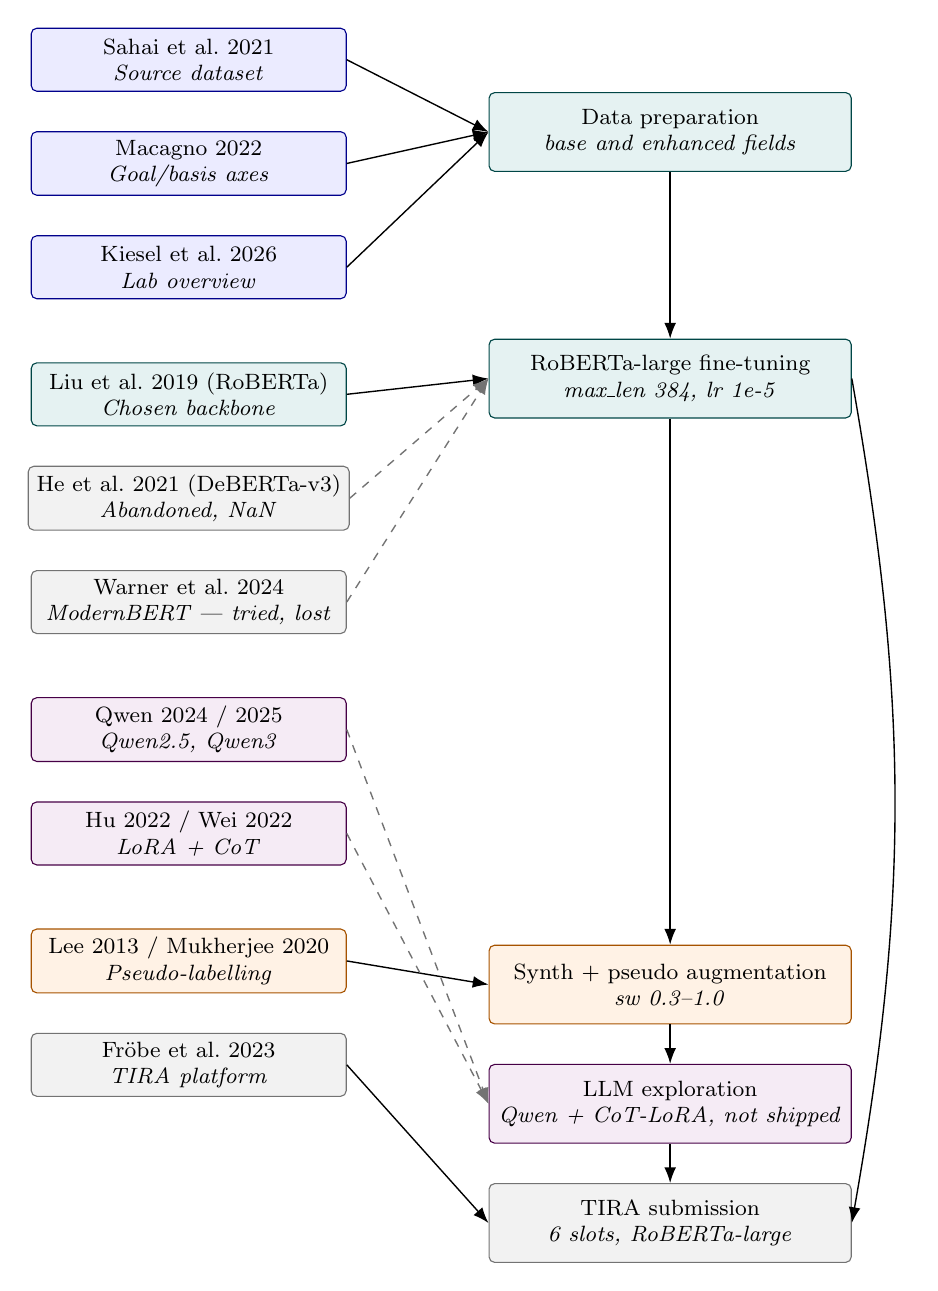
\begin{tikzpicture}[
  node distance = 5mm and 18mm,
  font          = \footnotesize,
  every node/.style = {align=center},
  citebox/.style = {draw, rounded corners=2pt, inner sep=3pt,
                    minimum width=40mm, minimum height=8mm,
                    line width=0.4pt},
  pipebox/.style = {draw, rounded corners=2pt, inner sep=3pt,
                    minimum width=46mm, minimum height=10mm,
                    line width=0.4pt},
  blue/.style   = {citebox, fill=blue!8,   draw=blue!55!black},
  teal/.style   = {citebox, fill=teal!10,  draw=teal!55!black},
  gray/.style   = {citebox, fill=black!5,  draw=black!55},
  purp/.style   = {citebox, fill=violet!8, draw=violet!55!black},
  amber/.style  = {citebox, fill=orange!10,draw=orange!65!black},
  ptl/.style    = {pipebox, fill=teal!10,  draw=teal!55!black},
  pgr/.style    = {pipebox, fill=black!5,  draw=black!55},
  pam/.style    = {pipebox, fill=orange!10,draw=orange!65!black},
  ppu/.style    = {pipebox, fill=violet!8, draw=violet!55!black},
  solid/.style  = {-{Latex[length=2mm]}, line width=0.5pt},
  dropped/.style= {-{Latex[length=2mm]}, line width=0.5pt, dashed,
                   draw=black!55},
]

% Left column: citations
\node[blue]  (c1)                            {Sahai et al.\ 2021\\\textit{Source dataset}};
\node[blue,  below=of c1] (c2)               {Macagno 2022\\\textit{Goal/basis axes}};
\node[blue,  below=of c2] (c3)               {Kiesel et al.\ 2026\\\textit{Lab overview}};
\node[teal,  below=8mm of c3] (c4)           {Liu et al.\ 2019 (RoBERTa)\\\textit{Chosen backbone}};
\node[gray,  below=of c4] (c5)               {He et al.\ 2021 (DeBERTa-v3)\\\textit{Abandoned, NaN}};
\node[gray,  below=of c5] (c6)               {Warner et al.\ 2024\\\textit{ModernBERT --- tried, lost}};
\node[purp,  below=8mm of c6] (c7)           {Qwen 2024 / 2025\\\textit{Qwen2.5, Qwen3}};
\node[purp,  below=of c7] (c8)               {Hu 2022 / Wei 2022\\\textit{LoRA + CoT}};
\node[amber, below=8mm of c8] (c9)           {Lee 2013 / Mukherjee 2020\\\textit{Pseudo-labelling}};
\node[gray,  below=of c9] (c10)              {Fr\"{o}be et al.\ 2023\\\textit{TIRA platform}};

% Right column: pipeline
\node[ptl, right=of c2, yshift=4mm]   (p1) {Data preparation\\\textit{base and enhanced fields}};
\node[ptl, right=of c4, yshift=2mm]   (p2) {RoBERTa-large fine-tuning\\\textit{max\_len 384, lr 1e-5}};
\node[pam, right=of c9, yshift=-3mm]  (p3) {Synth + pseudo augmentation\\\textit{sw 0.3--1.0}};
\node[ppu, below=of p3]               (p4) {LLM exploration\\\textit{Qwen + CoT-LoRA, not shipped}};
\node[pgr, below=of p4]               (p5) {TIRA submission\\\textit{6 slots, RoBERTa-large}};

% Edges: chosen routes
\draw[solid] (c1.east) -- (p1.west);
\draw[solid] (c2.east) -- (p1.west);
\draw[solid] (c3.east) -- (p1.west);
\draw[solid] (c4.east) -- (p2.west);
\draw[solid] (c9.east) -- (p3.west);
\draw[solid] (c10.east) -- (p5.west);

% Edges: dropped routes
\draw[dropped] (c5.east) -- (p2.west);
\draw[dropped] (c6.east) -- (p2.west);
\draw[dropped] (c7.east) -- (p4.west);
\draw[dropped] (c8.east) -- (p4.west);

% Internal flow on the right
\draw[solid] (p1.south) -- (p2.north);
\draw[solid] (p2.south) -- (p3.north);
\draw[solid] (p3.south) -- (p4.north);
\draw[solid] (p4.south) -- (p5.north);
\draw[solid] (p2.east) to[bend left=10] (p5.east);

\end{tikzpicture}
\caption{Which prior work fed which component of our pipeline. Solid
arrows are routes that shipped; dashed arrows are routes we tried
and dropped (DeBERTa-v3-large under NaN, ModernBERT-large
underperforming RoBERTa-large, and the LLM alternative that did not
out-perform RoBERTa-large under cross-validation within our compute
envelope).}
\label{fig:citgraph}
\end{figure}

\end{document}
